\documentclass{article}

% if you need to pass options to natbib, use, e.g.:
% \PassOptionsToPackage{numbers, compress}{natbib}
% before loading nips_2017
%
% to avoid loading the natbib package, add option nonatbib:
% \usepackage[nonatbib]{nips_2017}

\usepackage[final]{nips_2017}

% to compile a camera-ready version, add the [final] option, e.g.:
% \usepackage[final]{nips_2017}

\usepackage[utf8]{inputenc} % allow utf-8 input
\usepackage[T1]{fontenc}    % use 8-bit T1 fonts
\usepackage{hyperref}       % hyperlinks
\usepackage{url}            % simple URL typesetting
\usepackage{booktabs}       % professional-quality tables
\usepackage{amsfonts}       % blackboard math symbols
\usepackage{nicefrac}       % compact symbols for 1/2, etc.
\usepackage{microtype}      % microtypography
\usepackage{cite}
\usepackage{amsmath}
\usepackage{graphicx} 

\usepackage{algorithm}  
\usepackage{algpseudocode}  
\usepackage{amsmath}  
\renewcommand{\algorithmicrequire}{\textbf{Input:}}  % Use Input in the format of Algorithm  
\renewcommand{\algorithmicensure}{\textbf{Output:}} % Use Output in the format of Algorithm  

\hypersetup{colorlinks,linkcolor={blue},citecolor={blue},urlcolor={blue}}  

\title{CS150A Database \\Course Project}

% The \author macro works with any number of authors. There are two
% commands used to separate the names and addresses of multiple
% authors: \And and \AND.
%
% Using \And between authors leaves it to LaTeX to determine where to
% break the lines. Using \AND forces a line break at that point. So,
% if LaTeX puts 3 of 4 authors names on the first line, and the last
% on the second line, try using \AND instead of \And before the third
% author name.

\author{
  Yuhan Cao\\
  ID: 2020533165\\
  \texttt{caoyh1@shanghaitech.edu.cn} \\
  %% examples of more authors
   \And
  Zhenbang LI\\
  ID: 2019531055\\
  \texttt{lizhb@shanghaitech.edu.cn}
}

\begin{document}
% \nipsfinalcopy is no longer used

\maketitle

\begin{abstract}
This project is intended to predict student performance on mathematical problems from logs of
student interaction with Intelligent Tutoring Systems. This task presents interesting technical
challenges, has practical importance, and is scientifically interesting. In this project, we follow the 5 suggested steps for building a practical machine learning system and implemented with \textbf{\textit{Pyspark}}, which is also the structure title of this report.
\end{abstract}

\section{Explore the dataset}
The training dataset is composed of 19 features (Or 20, if consider\textit{ Problem Hierarchy} as a combination of unit and section.), which can be classified into two groups: \\
\textbf{1. numerical features:}\\
Problem View, First Transaction Time, Correct Transaction Time, Step End Time, Step Duration (sec), Correct Step Duration (sec), Error Step Duration (sec), Correct First Attempt, Incorrects, Hints, Corrects, KC(Default), Opportunity(Default).	\\
\textbf{2. category features:}\\
Anon Student Id, Problem Hierarchy, Problem Name, Step Name.\\
After the adequate conversion, the types of the features are:

\begin{center} 
\centering
\begin{tabular}{|l|l|l|l|l|}
\hline 
Row&Anon Student Id&Problem Hierarchy&Problem Name &Problem View\\
\hline  
int64 & object & object & object & int64 \\
\hline 
Step Name& Step Start Time &First Transaction Time &Correct Transaction Time&Step End Time\\
\hline  
object & object & object & object & object \\
\hline 
Step Duration& Correct Step Duration &Error Step Duration &Correct First Attempt Time&Incorrects\\
\hline  
float64 & float64 & float64 & int64 & int64 \\
\hline 
Hints& Corrects &KC(Default) &Opportunity(Default) &NaN\\
\hline  
int64 & int64 & object & object & NaN \\
\hline 
\end{tabular}\\
\textbf{Fig1. Data types of the features}\\
\end{center}
As shown below, Fig2 is a visualization of the distribution of major features.\\\\
However, the testing dataset contains only the 6 category features: \textit{Anon Student Id}, \textit{Problem Hierarchy}, \textit{Problem Name}, \textit{Problem Unit}, \textit{Problem Section}, \textit{Step Name}, which should be emphasised in our training dataset. The testing dataset have some invalid and  missing entries that should be cleaned in 1140 rows.\\

\section{Data cleaning}
The target of prediction is the Correct First Attempt (CFA). So instead of evenly considering the relations between the components, we should focus on the relations between each other component and CFA. What's more, there are considerable amount of missing of corresponding CFA, in which case we take the mean CFA of the other same-type elements as the complement. For these category components, we take a modified one-hot encoding. In this way, we generate the corresponding \textit{feature-CFA} of the \textit{Anon Student Id,} \textit{Problem Name}, \textit{Step Name}, which together with other components construct the training dataset.\\

\section{Feature engineering}
As mentioned in the above section, we add the \textit{feature-CFA} relations as new features. To achieve this relation feature, first we should group the dataframe by the original target feature, then filter out those entries without the correct first attempt mark equals 1. For those missing values (entries with correct first attempt = 0), we will take the mean of the other \textit{target feature-CFA} values.\\
In this way, we quantize a distinct relation between each feature and CFA, reduce the information loss cost by the correlation between features. In our test, these additional features improve the accuracy of prediction, especially for the tree based models.

\graphicspath{ {./images/} }
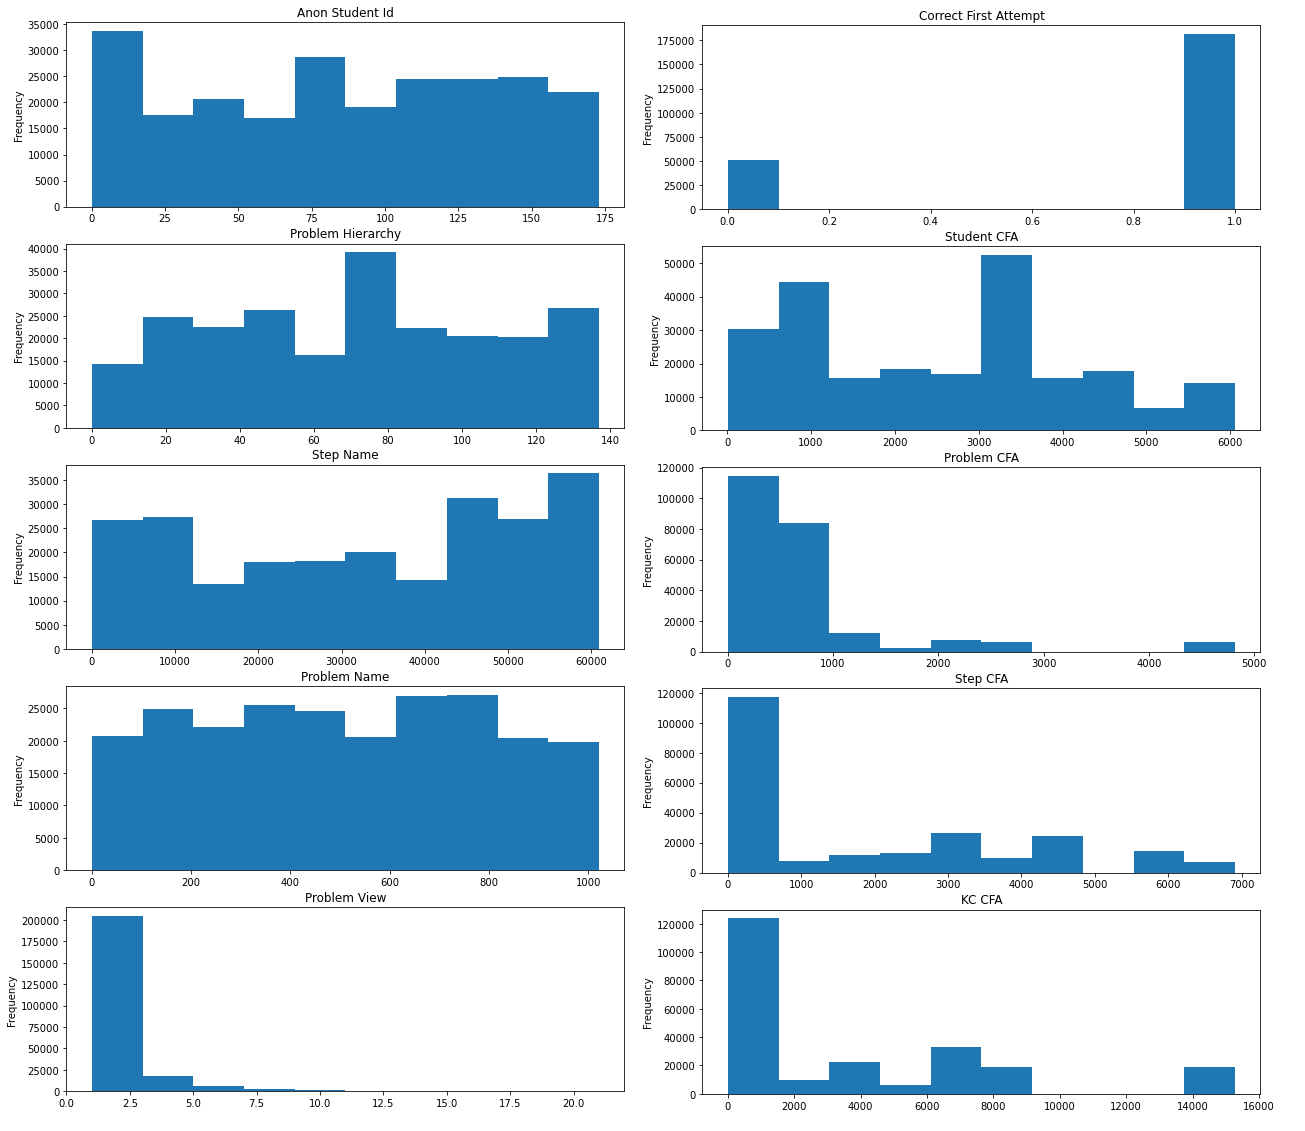
\includegraphics[scale=0.85]{distribution}
\begin{center} 
\centering
\textbf{Fig2. distribution of cleaned and encoded features}\\
\end{center}

\section{Learning algorithm}
We perform 6 algorithms, including both tree based ones and neural network based ones:\\\\
(1) Decision Tree:  We choose the naive decision tree as a baseline.\\
(2) Random Forest:  We choose it as a baseline for tuning.\\
(3) AdaBoost Regressor:  AdaBoost is adaptive in the sense that subsequent weak learners are tweaked in favor of those instances misclassified by previous classifiers. In some problems it can be less susceptible to the overfitting problem than other learning algorithms.\\
(4) Logistic Regression:  We choose the logistic regression as a baseline and comparison.\\
(5) LSTM:  LSTM networks are well-suited to classifying, processing and making predictions based on time series data, since there can be lags of unknown duration between important events in a time series, which is suitable for our case.\\
(6) LightGBM:  Gradient boosting based models have the first tier performance among the tree based classes. LightGBM is a efficient one and relatively easy to tun.\\\\
Consider the feature number and size of training set (23744) and testing set (1140), the over-fitting can become the major potential problem for neural network based methods. So we also focus on the tree based algorithm, especially the lightGBM, which turns out to be good after tuning the hyperparameters.

\section{Hyperparameter selection and model performance}
After training the models on their original hyperparameters and compare the results, we chose the models that have the most potential. We mainly tuned 2 models: LSTM and lightGBM.\\
Our LSTM is implemented based on \textit{keras} and  have 3 layer, batch size 32 and epoch 10, the tuning of hyperparameters does not have a satifying outcome. The over-fitting may be the major problem since the dimension of the features is limited.\\
For the lightGBM, we increase the n-estimator (number of boosted trees to fit) to 1000, and correspondingly decrease the n-eaves (maximum tree leaves for base learners), considering the uneven distribution of out training dataset. In addtion, to reduce over-fitting, we add the sub samples which can help specify the percentage of rows used per tree building iteration. That means some rows will be randomly selected for fitting each learner (tree). The ratio and frequency of sub samples are tuned in range to find the best result.  Fig3 is a table of the major hyperparameters of our lightGBM after tuning.\\
\begin{center} 
\centering
\begin{tabular}{|l|l|l|l|l|l|}
\hline 
max-depth&num-leaves&learning-rate&n-estimators&min-child-samples&subsample\\
\hline  
5 & 20 & 0.1 & 1000 & 20 & 0.85\\
\hline 
subsample-freq&boost-from-average&reg-lambda&verbose&boosting-type&n-jobs\\
\hline  
1 & false & 0.1 & -1 & gbdt & -1\\
\hline 
\end{tabular}\\
\textbf{Fig3. Chosen hyperparameters of lightGBM}\\
\end{center}

The final result of our models:

\begin{center} 
\centering
\begin{tabular}{ll}
\hline
Model & RMSE\\
\hline
Decision Tree & 0.5126039 \\
Random Forest & 0.4165785 \\
AdaBoost Regressor & 0.4276248 \\
Logistic Regression & 0.4198125 \\
LSTM & 0.4227168 \\
LSTM (tuned) & 0.4121097 \\
LightGBM & 0.4102617 \\
LightGBM (tuned) & 0.3970613 \\
Best RMSE & 0.3970613\\
\hline
\end{tabular}\\
\textbf{Fig4. Performance of the models}\\
\end{center}

\section{PySpark implementation (optional)}
In the data cleaning and feature engineering process, we need to compute the mean value of the features for complement purpose. We operate a SparkSession and crete SQL views for cleaning the train dataset.
\end{document}
\printbibliography{}
